% board-warping-lenses/bw_ag_tamron.tex — generated by board-warping-lenses/tools/board_warping_lenses.py; do not edit.
% One 3-D panel: the estimated height field of set bw_ag_tamron as a surface over the page (979 x 979 mm; x to the right, y up the page,
% z the height in mm, towards the camera), spline camera, refine product 1613c14e5a386dd0. 5 x 5 mesh points; every patch has
% the colour of its band (0.5 mm). Orthographic view (azimuth 20, elevation 38 degrees) with the heights 50 times as large as
% lengths on the page: the axis' height is chosen so that PGFPlots' filling of width x height is exactly that projection. The box is
% -3 ... +3 mm in every panel. Its width is \rcpanelwidth, of which 10 pt at the left hold the tick labels.
\providecommand{\rcfigdir}{src/fig}%
\providecommand{\rcpanelwidth}{\linewidth}%
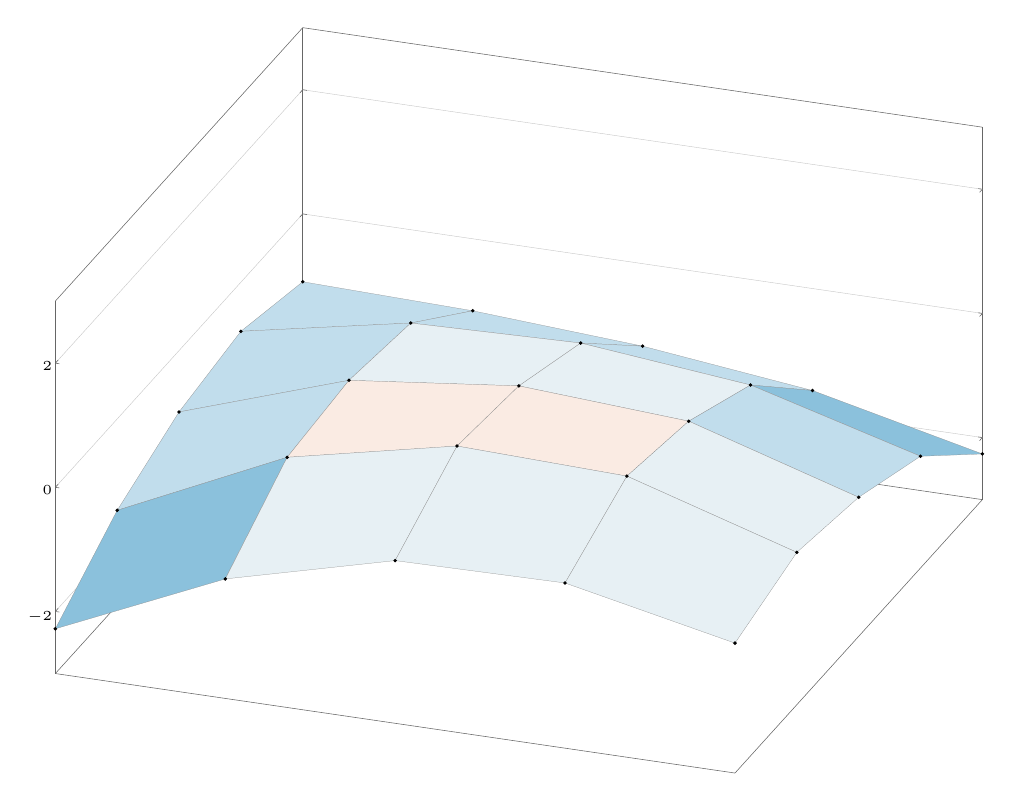
\begin{tikzpicture}[baseline=(current axis.center)]
\pgfmathsetlengthmacro{\rcwarpw}{\rcpanelwidth-10pt}%
\begin{axis}[
  scale only axis, width=\rcwarpw, height=0.80406*\rcwarpw, view={20}{38},
  xmin=0, xmax=979.0, ymin=0, ymax=979.0, zmin=-3, zmax=3, clip=false,
  xtick=\empty, ytick=\empty, ztick={-2,0,2}, zticklabel style={font=\tiny, inner sep=1pt},
  tick style={line width=0.2pt, black!60}, major tick length=1.5pt, zmajorgrids, grid style={line width=0.15pt, black!22},
  axis line style={line width=0.2pt, black!60},
  colormap={warp}{rgb255=(17,71,128) rgb255=(42,113,178) rgb255=(74,151,197) rgb255=(139,193,220) rgb255=(193,221,236) rgb255=(231,240,244) rgb255=(250,235,227) rgb255=(251,206,182) rgb255=(241,159,126) rgb255=(216,102,81) rgb255=(187,42,52) rgb255=(134,10,36)}, colormap access=piecewise const, point meta min=-3, point meta max=3]
\addplot3[surf, shader=faceted, faceted color=black!45, line width=0.08pt, mesh/rows=5, z buffer=sort, point meta=z] coordinates {
(0.0,0.0,-2.279) (244.8,0.0,-1.075) (489.5,0.0,-0.379) (734.2,0.0,-0.339) (979.0,0.0,-0.907)
(0.0,244.8,-1.472) (244.8,244.8,-0.217) (489.5,244.8,0.365) (734.2,244.8,0.281) (979.0,244.8,-0.546)
(0.0,489.5,-0.988) (244.8,489.5,-0.078) (489.5,489.5,0.233) (734.2,489.5,0.065) (979.0,489.5,-0.760)
(0.0,734.2,-0.790) (244.8,734.2,-0.256) (489.5,734.2,-0.178) (734.2,734.2,-0.453) (979.0,734.2,-1.200)
(0.0,979.0,-1.093) (244.8,979.0,-1.160) (489.5,979.0,-1.329) (734.2,979.0,-1.643) (979.0,979.0,-2.264)
};
\addplot3[only marks, mark=*, mark size=0.4pt, black] coordinates {(0.0,979.0,-1.093) (244.8,979.0,-1.160) (489.5,979.0,-1.329) (734.2,979.0,-1.643) (979.0,979.0,-2.264) (0.0,734.2,-0.790) (244.8,734.2,-0.256) (489.5,734.2,-0.178) (734.2,734.2,-0.453) (979.0,734.2,-1.200) (0.0,489.5,-0.988) (244.8,489.5,-0.078) (489.5,489.5,0.233) (734.2,489.5,0.065) (979.0,489.5,-0.760) (0.0,244.8,-1.472) (244.8,244.8,-0.217) (489.5,244.8,0.365) (734.2,244.8,0.281) (979.0,244.8,-0.546) (0.0,0.0,-2.279) (244.8,0.0,-1.075) (489.5,0.0,-0.379) (734.2,0.0,-0.339) (979.0,0.0,-0.907)};
\end{axis}
\pgfresetboundingbox\path ([xshift=-10pt]current axis.south west) rectangle (current axis.north east);   % the box is the axis and the strip of the tick labels
\end{tikzpicture}%
